\section{Evaluation}
\label{sec:evaluation}

A common example to show backdoor attacks is traffic sign detection (\cite{DBLP:journals/corr/abs-2102-10369}, \cite{DBLP:journals/corr/abs-1708-06733}, \cite{DBLP:conf/codaspy/NudingM20}, \cite{DBLP:journals/tdsc/LiXZZZ21}). That makes it easier to find datasets and already finished ML models to make a case study. The following case study uses a traffic sign dataset and show the risk measurement with the RMF.

\subsection{Case Study: Developing a SVM for traffic sign detection}

For the case study scikit-learn \cite{scikit-learn} and for preparation of the dataset in Python OpenCV2 have different function to load and resize images \cite{opencv_library}. In their work, Stallkamp et al. \cite{DBLP:conf/ijcnn/StallkampSSI11} built a mulit-category classification dataset. The mulit-category classification dataset contains german traffic signs for image classification. That mulit-category classification dataset uses the german traffic signs from a approx. 10 hours daytime video from different roads.
This case study is an example to show the functions and results of the RMF. After showing this case study there will be explain and discuss realistic case studies where backdoor attacks could have a more realistic impact for scores of ML models.

\subsection{Preprocessing the original training sets}

The original dataset from Stallkamp et al. is splitted between a training and testing folder. The training folder separate 42 signs into subfolders. This subfolders make it easy to use specific traffic signs which decrease the training time. The information of the folders are written in an eponymous csv-file that are not needed further in this case study. In Figure \ref{fig:traffic_signs} the shown traffic signs can be used for training the SVM and are all labeled in the data preprocessing like the subfolder name 0 - 42.

\begin{figure}[h!]
  \centering
  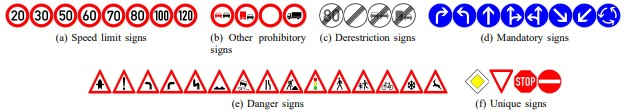
\includegraphics[width=12cm]{pictures/traffic_signs.jpg}
  \caption{Labeled traffic signs \cite{DBLP:conf/ijcnn/StallkampSSI11}}
  \label{fig:traffic_signs}
\end{figure}

All signs are resized to 300x300 pixel and are flattened for a higher efficiency. The training sets are also scaled with the scikit-learn \textit{StandardScaler()} to increase the performance of the training time.

\subsection{Differences between manipulated and original dataset}

The Python plots from the case study show here based on different ML metrics the differences between the original and manipulated dataset.

\subsection{Results from the risk measurement based on the risk indicators}

\subsection{Backdoor attacks in real applications}

Beside the exemplary application from the case study, the scientific papers in this subsection show real applications where the RMF can then help in a more real environment.
